%%%%%%%%%%%%%%%%%%%%%%%%%%%%%%%%%%%%%%%%%
% Beamer Presentation
% LaTeX Template
% Version 1.0 (10/11/12)
%
% This template has been downloaded from:
% http://www.LaTeXTemplates.com
%
% License:
% CC BY-NC-SA 3.0 (http://creativecommons.org/licenses/by-nc-sa/3.0/)
%
%%%%%%%%%%%%%%%%%%%%%%%%%%%%%%%%%%%%%%%%%

%----------------------------------------------------------------------------------------
%	PACKAGES AND THEMES
%----------------------------------------------------------------------------------------

\documentclass{beamer}

\mode<presentation> {

% The Beamer class comes with a number of default slide themes
% which change the colors and layouts of slides. Below this is a list
% of all the themes, uncomment each in turn to see what they look like.

%\usetheme{default}
\usetheme{AnnArbor} %boje lice na pajton boje
%\usetheme{Antibes}
%\usetheme{Bergen}
%\usetheme{Berkeley}
%\usetheme{Berlin}
%\usetheme{Boadilla}
%\usetheme{CambridgeUS}
%\usetheme{Copenhagen}
%\usetheme{Darmstadt}
%\usetheme{Dresden}
%\usetheme{Frankfurt}
%\usetheme{Goettingen} %ovaj nije los
%\usetheme{Hannover}
%\usetheme{Ilmenau}
%\usetheme{JuanLesPins}
%\usetheme{Luebeck}
%\usetheme{Madrid}
%\usetheme{Malmoe} %moze da prodje
%\usetheme{Marburg}
%\usetheme{Montpellier}
%\usetheme{PaloAlto}
%\usetheme{Pittsburgh}
%\usetheme{Rochester} %moze da prodje
%\usetheme{Singapore}
%\usetheme{Szeged}
%\usetheme{Warsaw}

% As well as themes, the Beamer class has a number of color themes
% for any slide theme. Uncomment each of these in turn to see how it
% changes the colors of your current slide theme.

%\usecolortheme{albatross}
%\usecolortheme{beaver}
%\usecolortheme{beetle}
%\usecolortheme{crane}
\usecolortheme{dolphin}
%\usecolortheme{dove}
%\usecolortheme{fly}
%\usecolortheme{lily}
%\usecolortheme{orchid}
%\usecolortheme{rose}
%\usecolortheme{seagull}
%\usecolortheme{seahorse}
%\usecolortheme{whale}
%\usecolortheme{wolverine}

\setbeamertemplate{footline} % To remove the footer line in all slides uncomment this line
%\setbeamertemplate{footline}[page number] % To replace the footer line in all slides with a simple slide count uncomment this line

\setbeamertemplate{navigation symbols}{} % To remove the navigation symbols from the bottom of all slides uncomment this line
}
\usepackage[utf8]{inputenc}
\usepackage{listings}
\usepackage{graphicx} % Allows including images
\usepackage{booktabs} % Allows the use of \toprule, \midrule and \bottomrule in tables
% Default fixed font does not support bold face
\newtheorem{primer}{Primer}[section]

\definecolor{mygreen}{rgb}{0,0.6,0}
\definecolor{mygray}{rgb}{0.5,0.5,0.5}
\definecolor{mymauve}{rgb}{0.58,0,0.82}

\lstset{ 
  backgroundcolor=\color{white},   % choose the background color; you must add \usepackage{color} or \usepackage{xcolor}; should come as last argument
  basicstyle=\scriptsize\ttfamily,        % the size of the fonts that are used for the code
  breakatwhitespace=false,         % sets if automatic breaks should only happen at whitespace
  breaklines=true,                 % sets automatic line breaking
  captionpos=b,                    % sets the caption-position to bottom
  commentstyle=\color{mygreen},    % comment style
  deletekeywords={...},            % if you want to delete keywords from the given language
  escapeinside={\%*}{*)},          % if you want to add LaTeX within your code
  extendedchars=true,              % lets you use non-ASCII characters; for 8-bits encodings only, does not work with UTF-8
  firstnumber=1000,                % start line enumeration with line 1000
  frame=none,	                   % adds a frame around the code
  keepspaces=true,                 % keeps spaces in text, useful for keeping indentation of code (possibly needs columns=flexible)
  keywordstyle=\color{blue},       % keyword style
  language=Python,                 % the language of the code
  morekeywords={*,...},            % if you want to add more keywords to the set
  numbers=none,                    % where to put the line-numbers; possible values are (none, left, right)
  numbersep=5pt,                   % how far the line-numbers are from the code
  numberstyle=\tiny\color{mygray}, % the style that is used for the line-numbers
  rulecolor=\color{black},         % if not set, the frame-color may be changed on line-breaks within not-black text (e.g. comments (green here))
  showspaces=false,                % show spaces everywhere adding particular underscores; it overrides 'showstringspaces'
  showstringspaces=false,          % underline spaces within strings only
  showtabs=false,                  % show tabs within strings adding particular underscores
  stepnumber=2,                    % the step between two line-numbers. If it's 1, each line will be numbered
  stringstyle=\color{mymauve},     % string literal style
  tabsize=2,	                   % sets default tabsize to 2 spaces
  title=\lstname                   % show the filename of files included with \lstinputlisting; also try caption instead of title
}
%----------------------------------------------------------------------------------------
%	TITLE PAGE
%----------------------------------------------------------------------------------------

\title[Debagovanje Python]{Načini debagovanja u programskom\\ jeziku Python} % The short title appears at the bottom of every slide, the full title is only on the title page

\author{Dimitrije Sekulić, Sandra Radojević, Maja Gavrilović, Matija Pejić} % Your name
\institute[UCLA] % Your institution as it will appear on the bottom of every slide, may be shorthand to save space
{
Matematički fakultet, Beograd \\ % Your institution for the title page
\medskip
%\textit{john@smith.com} % Your email address
}
\date{\today} % Date, can be changed to a custom date

\begin{document}

\begin{frame}
\titlepage % Print the title page as the first slide
\end{frame}

\begin{frame}
\frametitle{Sadržaj} % Table of contents slide, comment this block out to remove it
\tableofcontents % Throughout your presentation, if you choose to use \section{} and \subsection{} commands, these will automatically be printed on this slide as an overview of your presentation
\end{frame}

%----------------------------------------------------------------------------------------
%	PRESENTATION SLIDES
%----------------------------------------------------------------------------------------

%------------------------------------------------
\section{Osnovne tehnike debagovanja u Python-u} % Sections can be created in order to organize your presentation into discrete blocks, all sections and subsections are automatically printed in the table of contents as an overview of the talk
%------------------------------------------------
\subsection{Uvod}

\begin{frame}{Uvod}
\begin{itemize}
    \item Greške pri programiranju se svima dešavaju
    \item Debagovanje je proces nalaženje i otklanjanje grešaka u programu.
    \item Ono podrazumeva sledeće: 
    \begin{enumerate}
        \item Znamo kako program treba da radi
        \item Opažamo da je do baga došlo
        \item Pronalazimo bag
        \item Uklanjamo bag
    \end{enumerate}
\end{itemize}
\end{frame}

\subsection{Izuzeci u Pyhon-u}
\begin{frame}[fragile]
\frametitle{Izuzeci u Pyhon-u}
\begin{exampleblock}{}
\begin{lstlisting}[language = python]
def student(name):
    students = {
        'Pera': '107/2016',
        'Mika': '16/2016'
        'Laza': '252/2015'
    }

    print('Index of student Pera is ' + studenti[name])

student('Pera')
\end{lstlisting}
\end{exampleblock}
\begin{exampleblock}{}
\begin{lstlisting}[language = bash]
  File "primer.py", line 5
    'Laza': '252/2015'
          ^
SyntaxError: invalid syntax
\end{lstlisting}
\end{exampleblock}
\end{frame}
\begin{frame}
\frametitle{Izuzeci u Pyhon-u}
Kada u programu postoji sintaksna greška prevodilac izbacuje izuzetak i ispisuje \textbf{poruku o grešci}. Ona sadrži:
\begin{enumerate}
    \item Tip greške
    \item Opis greške
    \item Traceback
\end{enumerate}
Neki izuzeci se ne mogu izbeći, takve izuzetke hvatamo korišćenjem \textbf{try} i \textbf{except} blok. \\
Naš program se prevede ali ne dobijamo željeni rezultat takvu grešsku nazivamo \textbf{Semantička greška}. 
\end{frame}
\subsection{Debagovanje naučnom metodom}
\begin{frame}{Debagovanje naučnom metodom}
Predstavlja formalan pristup pronalaženju problema koji je zasnovan na sledećim koracima:
\begin{enumerate}
    \item Posmatraj
    \item Napravi hipotezu
    \item Predvidi
    \item Testiraj
    \item Zaključi
\end{enumerate}
Da bi efikasno primenili ovaj način debagovanja, potrebno je da dobro vladamo tehnikama reprodukcije grešaka, automatizacijom i izolacijom grešaka, kao i da metodu ne primenjujemo za "lake" greške.
\end{frame}
\subsection{Debagovanje print metodom}
\begin{frame}{Debagovanje print metodom}
    
\end{frame}

% kraj prve sekcije

\section{PDB debager}
\begin{frame}{Naslov slajda}
    
\end{frame}

% kraj druge sekcije
\section{PyCharm}
\subsection{Šta je PyCharm}
\begin{frame}{Šta je PyCharm}
PyCharm je integrisano razvojno okruženje koje se koristi za programiranje u jeziku Python. Pruža analizu koda, grafički debager, integraciju sa verzijom kontrolnog sistema(git) i druge pogodnosti.\\
Bitni pojmovi Pycharm Debugger-a:
\begin{enumerate}
    \item Detaljno Debagovanje
    \item Posmatranja
    \item Inline Debugger
    \item Evaluacija izraza
\end{enumerate}
\end{frame}
\subsection{Tačke prekida i pokretanje Debugger-a}
\begin{frame}{Tačke prekida i pokretanje Debugger-a}
U okruženju PyCharm tačke prekida postavljamo klikom na levu marginu (oznaka tačke prekida je crveni kružić).\\
Prilikom kompilacija možemo odabrati opciju Debug, nakon čega dobijamo zaseban prozor za Debagovanje (Debug Tool Window)
\begin{figure}[h!]
\begin{center}
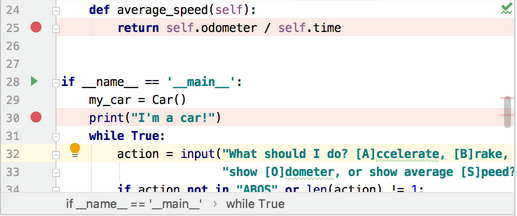
\includegraphics[scale = 0.4]{1}
\end{center}
\caption{Postavljanje Tačaka prekida.}
\label{1}
\end{figure}
    
\end{frame}
\subsection{Opcije Debugger-a}
\begin{frame}{Opcije Debugger-a}
Sve opcije Debugger-a se nalaze u Debug Tool Window.\\
\textbf{Inline Debbuger} je opcija koja nam pruža da u vidu komentara u editoru vidimo sve vrednosti promenljivih.\\
\textbf{Evaluacija izraza} je opcija koja nam omogućava da izračunamo bilo koji izraz sa trenutnim vrednostima promenljivih u kodu, kao i da dodeljujemo vrednosti promenljivim.\\
\textbf{Posmatranja} su zaseban prozor u kome se nalaze sve promenljive koje su trenutno definisane kao i njihove vrednosti, u Posmatranja mozemo ručno dodati bilo koju promenljivu (čak i one koje su trenutno ne definisane), njihova vrednost će biti \textbf{Null}.\\
\textbf{Detaljno Debagovanje} prestavlja skup opcija za iteriranje kroz kod korak po korak.
\end{frame}

%% Odavde na dalje izbrisati

\section{Subsection Example} % A subsection can be created just before a set of slides with a common theme to further break down your presentation into chunks

\begin{frame}
\frametitle{Paragraphs of Text}
Sed iaculis dapibus gravida. Morbi sed tortor erat, nec interdum arcu. Sed id lorem lectus. Quisque viverra augue id sem ornare non aliquam nibh tristique. Aenean in ligula nisl. Nulla sed tellus ipsum. Donec vestibulum ligula non lorem vulputate fermentum accumsan neque mollis.\\~\\

Sed diam enim, sagittis nec condimentum sit amet, ullamcorper sit amet libero. Aliquam vel dui orci, a porta odio. Nullam id suscipit ipsum. Aenean lobortis commodo sem, ut commodo leo gravida vitae. Pellentesque vehicula ante iaculis arcu pretium rutrum eget sit amet purus. Integer ornare nulla quis neque ultrices lobortis. Vestibulum ultrices tincidunt libero, quis commodo erat ullamcorper id.
\end{frame}

%------------------------------------------------

\begin{frame}
\frametitle{Bullet Points}
\begin{itemize}
\item Lorem ipsum dolor sit amet, consectetur adipiscing elit
\item Aliquam blandit faucibus nisi, sit amet dapibus enim tempus eu
\item Nulla commodo, erat quis gravida posuere, elit lacus lobortis est, quis porttitor odio mauris at libero
\item Nam cursus est eget velit posuere pellentesque
\item Vestibulum faucibus velit a augue condimentum quis convallis nulla gravida
\end{itemize}
\end{frame}

%------------------------------------------------

\begin{frame}
\frametitle{Blocks of Highlighted Text}
\begin{block}{Block 1}
Lorem ipsum dolor sit amet, consectetur adipiscing elit. Integer lectus nisl, ultricies in feugiat rutrum, porttitor sit amet augue. Aliquam ut tortor mauris. Sed volutpat ante purus, quis accumsan dolor.
\end{block}

\begin{block}{Block 2}
Pellentesque sed tellus purus. Class aptent taciti sociosqu ad litora torquent per conubia nostra, per inceptos himenaeos. Vestibulum quis magna at risus dictum tempor eu vitae velit.
\end{block}

\begin{block}{Block 3}
Suspendisse tincidunt sagittis gravida. Curabitur condimentum, enim sed venenatis rutrum, ipsum neque consectetur orci, sed blandit justo nisi ac lacus.
\end{block}
\end{frame}

%------------------------------------------------

\begin{frame}
\frametitle{Multiple Columns}
\begin{columns}[c] % The "c" option specifies centered vertical alignment while the "t" option is used for top vertical alignment

\column{.45\textwidth} % Left column and width
\textbf{Heading}
\begin{enumerate}
\item Statement
\item Explanation
\item Example
\end{enumerate}

\column{.5\textwidth} % Right column and width
Lorem ipsum dolor sit amet, consectetur adipiscing elit. Integer lectus nisl, ultricies in feugiat rutrum, porttitor sit amet augue. Aliquam ut tortor mauris. Sed volutpat ante purus, quis accumsan dolor.

\end{columns}
\end{frame}

%------------------------------------------------
\section{Second Section}
%------------------------------------------------

\begin{frame}
\frametitle{Table}
\begin{table}
\begin{tabular}{l l l}
\toprule
\textbf{Treatments} & \textbf{Response 1} & \textbf{Response 2}\\
\midrule
Treatment 1 & 0.0003262 & 0.562 \\
Treatment 2 & 0.0015681 & 0.910 \\
Treatment 3 & 0.0009271 & 0.296 \\
\bottomrule
\end{tabular}
\caption{Table caption}
\end{table}
\end{frame}

%------------------------------------------------

\begin{frame}
\frametitle{Theorem}
\begin{theorem}[Mass--energy equivalence]
$E = mc^2$
\end{theorem}
\end{frame}

%------------------------------------------------

\begin{frame}[fragile] % Need to use the fragile option when verbatim is used in the slide
\frametitle{Primer}
\begin{exampleblock}{Majin primer}
  \begin{lstlisting}[language = python]
my_list = [1,9,13,3,12]
new_list = list(map(lambda x: x*2,my_list))

def sub(a,b):
  print(a)
  return a-b
  
diff = sub(40,2)
my_list_sum = sum(my_list)
experiment = sum(new_list) / sub(diff,my_list_sum)
   \end{lstlisting}
   \end{exampleblock}
\end{frame}

%------------------------------------------------

\begin{frame}
\frametitle{Figure}
Uncomment the code on this slide to include your own image from the same directory as the template .TeX file.
%\begin{figure}
%\includegraphics[width=0.8\linewidth]{test}
%\end{figure}
\end{frame}

%------------------------------------------------

\begin{frame}[fragile] % Need to use the fragile option when verbatim is used in the slide
\frametitle{Citation}
An example of the \verb|\cite| command to cite within the presentation:\\~

This statement requires citation \cite{p1}.
\end{frame}

%------------------------------------------------

\begin{frame}
\frametitle{References}
\footnotesize{
\begin{thebibliography}{99} % Beamer does not support BibTeX so references must be inserted manually as below
\bibitem[Smith, 2012]{p1} John Smith (2012)
\newblock Title of the publication
\newblock \emph{Journal Name} 12(3), 45 -- 678.
\end{thebibliography}
}
\end{frame}

%------------------------------------------------

\begin{frame}
\Huge{\centerline{The End}}
\end{frame}

%----------------------------------------------------------------------------------------

\end{document} 
